% !TEX TS-program = pdflatex
% !TEX encoding = UTF-8 Unicode

% This is a simple template for a LaTeX document using the "article" class.
% See "book", "report", "letter" for other types of document.

\documentclass[11pt]{article} % use larger type; default would be 10pt

\usepackage[utf8]{inputenc} % set input encoding (not needed with XeLaTeX)

%%% Examples of Article customizations
% These packages are optional, depending whether you want the features they provide.
% See the LaTeX Companion or other references for full information.

%%% PAGE DIMENSIONS
\usepackage[a4paper,left=2cm,right=2cm,top=2cm,bottom=2cm]{geometry}
%\usepackage{geometry} % to change the page dimensions
% \geometry{a4paper} % or letterpaper (US) or a5paper or....
% \geometry{margin=0in} % for example, change the margins to 2 inches all round
% \geometry{landscape} % set up the page for landscape
%   read geometry.pdf for detailed page layout information

\usepackage{graphicx} % support the \includegraphics command and options

\usepackage[parfill]{parskip} % Activate to begin paragraphs with an empty line rather than an indent

%%% PACKAGES
\usepackage{booktabs} % for much better looking tables
\usepackage{array} % for better arrays (eg matrices) in maths
\usepackage{paralist} % very flexible & customisable lists (eg. enumerate/itemize, etc.)
\usepackage{verbatim} % adds environment for commenting out blocks of text & for better verbatim
\usepackage{subfig} % make it possible to include more than one captioned figure/table in a single float
\usepackage{amsmath}
\usepackage{amssymb}
\usepackage{logicproof}
\usepackage{tikz}
\usepackage{hyperref}
\usetikzlibrary{arrows,petri,topaths}
\usepackage{float}
\usepackage{graphicx}
\usepackage[T1]{fontenc}
\usepackage{listings}
\usepackage{pdflscape}
\lstset{
  basicstyle=\ttfamily,
  mathescape
}
% These packages are all incorporated in the memoir class to one degree or another...

%%% HEADERS & FOOTERS
\usepackage{fancyhdr} % This should be set AFTER setting up the page geometry
\pagestyle{fancy} % options: empty , plain , fancy
\renewcommand{\headrulewidth}{0pt} % customise the layout...
\lhead{}\chead{}\rhead{}
\lfoot{}\cfoot{\sffamily\thepage\normalfont}\rfoot{}

%%% SECTION TITLE APPEARANCE
\usepackage{sectsty}
\allsectionsfont{\sffamily\mdseries\upshape} % (See the fntguide.pdf for font help)
% (This matches ConTeXt defaults)

%%% ToC (table of contents) APPEARANCE
\usepackage[nottoc,notlof,notlot]{tocbibind} % Put the bibliography in the ToC
\usepackage[titles,subfigure]{tocloft} % Alter the style of the Table of Contents
\renewcommand{\cftsecfont}{\rmfamily\mdseries\upshape}
\renewcommand{\cftsecpagefont}{\rmfamily\mdseries\upshape} % No bold!
\newcommand{\qedsymbol}{\rightline{$\blacksquare$}}
\renewcommand{\familydefault}{\sfdefault}
\renewcommand{\thesection}{\hspace{-0.5cm}\arabic{section}}
\renewcommand{\thesubsection}{\alph{subsection})}
\renewcommand{\thesubsubsection}{Recursion depth \arabic{subsubsection}}

\usepackage[style=numeric-comp]{biblatex}

%%% END Article customizations

%%% The "real" document content comes below...

\title{\vspace{-1.6cm}Bioinformatics Assignment}
\author{zrlr73}
\date{} % Activate to display a given date or no date (if empty),
         % otherwise the current date is printed 

\begin{document}
\maketitle

\section{Markov Models}
\subsection{HMMs with silent states}
Since the Viterbi algorithm is already popular for solving this problem without silent states, I decided to adapt it forthe inclusion of silent states. The Viterbi algorithm iterates using the observed output of the modelled HMM, constructing a trellis of possible states for each observed output. Since we need to cater for states that do not provide any output whatsoever, we need to be able to generate possible silent states as well as the existing trellis of non-silent states. We also need to consider these silent states alongside the non-silent ones when deciding on possible precursors for each observed outcome.

Therefore, I would propose the following modified Viterbi algorithm:
\begin{lstlisting}
Initialise trellis with $v_0(0)=1, v_k(0)=0\quad|\quad k>0$
Initialise 2D array of linked list heads with size $m\times L$

// For each observed output
For $i=1\text{ to }L$ do:
  // For each possible state
  For each state $l$ do:
    $v_l(i) = e_l(x_i) \times max_k\{v_k(i-1)\times m_{kl}\}$

  // Evaluate possible silent states
  Initialise array $a$ of linked list heads with length $m$ and $a_0=v_l$
  Initialise numeric array $b$ with length $m$
  Integer j = 0
  Initialise Boolean value $loop$
  Do:
    j++
    loop = false
    For each state $s$ do:
      $a_j(s) = e_s($silent$)\times max_f\{a_{j-1}(f)\times m_{fs}\}$

      if ($a_j(s) > v_l(s)$ and $a_j(s) > a_{j-1}(s)$):
        loop = true
  While (loop)

\end{lstlisting}

\subsection{The Expectation-Maximisation Algorithm}
bruh



\section{Tree Reconstruction}

\subsection{The BUILD Algorithm}
If we call $(i,j)$ the lowest common ancestor of the leaves $i$ and $j$ of a tree, we can also define an operator $<$ which denotes the hierarchy of lowest common ancestors. For example, the constraint $(i,j)<(k,l)$ tells us that the lowest common ancestor of $k$ and $l$ is itself an ancestor of the lowest common ancestor of $i$ and $j$ - see figure below.

\begin{figure}
	\centering
	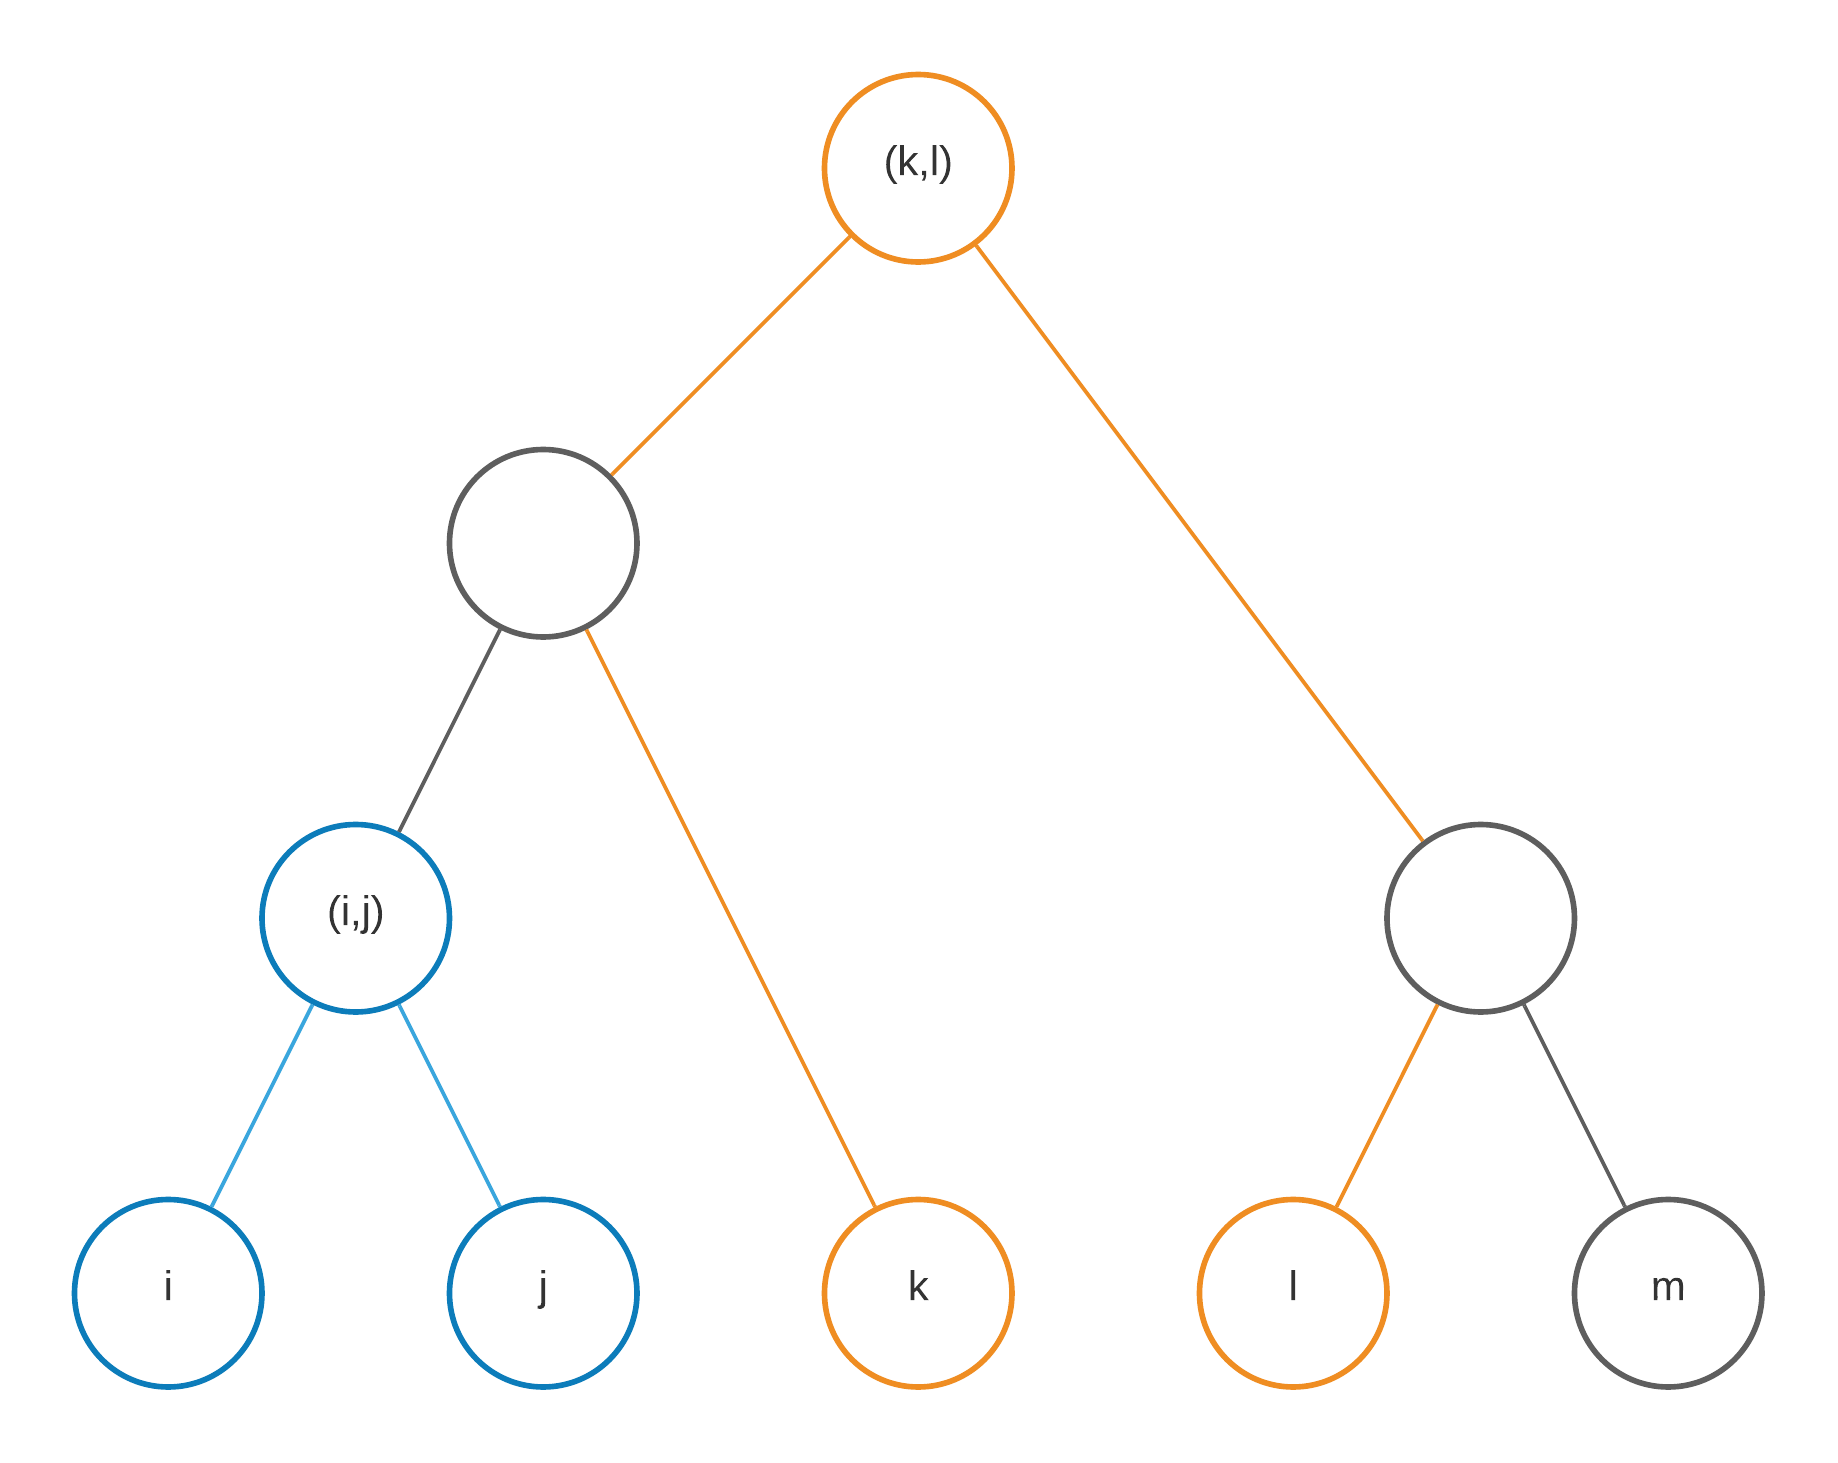
\includegraphics[width=10cm]{buildexample}
\end{figure}

The purpose of the BUILD algorithm is to construct a tree solely from these constraints. In a bioinformatics context, assuming the tree is a phylogeny, the constraints would be describing how closely related pairs of species are. As an example, we would specify the above constraint if we knew that the four species $\{i,j,k,l\}$ all had a common ancestor, but $i$ and $j$ were more closely related to each other than to the rest.

In BUILD, the structure of a tree is inferred using a technique known as 'partitioning'. This is when the set of leaves is split into groups known as 'blocks' at the root - for example, assuming descriptive enough constraints, the above tree would be split into the two sets $\{i,j,k\}$ and $\{l,m\}$. This partitioning can be done fairly easily using logical properties of the constraints:

From any constraint $(i,j)<(k,l)$ we can infer that:
\begin{enumerate}
	\item $i$ and $j$ are in the same block.
	\item If we already know that $k$ and $l$ are in the same block, then $i$ and $j$ must also be in that same block.
\end{enumerate}

We also assume that no two leaves are in the same block unless we can infer that they are from the constraints. In the original paper, this is the third rule.

With the set of leaves split into at least two blocks, we recurse into each block, partitioning every block until there is only one leaf left in the set. At this point, the algorithm's recursive structure exactly reflects the tree being constructed, so it simply needs to construct and return a tree. Instances with just one leaf return it, and instances that partitioned items join the returned structures with a new node until the outer layer is reached and the tree is complete.


\subsection{Partitioning}
Partitioning could occur as follows:
\begin{lstlisting}
// a 2D array: items in this array will be referred to as 'blocks'
$\pi_C$ = []

For each constraint $(a,b)<(c,d)$:
  If neither $a$ nor $b$ already exists in $\pi_C$:
    Add the new block [$a$,$b$] to $\pi_C$

  Else if $a$ and $b$ already exist in separate blocks in $\pi_C$:
    Replace those two blocks with their union

  Else if $a$ already exists in a block in $\pi_C$:
    Add $b$ to that block
  Else if $b$ already exists in a block in $\pi_C$:
    Add $a$ to that block

For each constraint $(a,b)<(c,d)$:
  If $c$ and $d$ share a block, merge the block containing $a$ and $b$ into it

For each leaf $x$ that is not a member of an existing block:
  Add the new block [$x$] to $\pi_C$
\end{lstlisting}

The result of this algorithm is the 2D array $\pi_C$, with structure as follows:
\begin{lstlisting}
[
  [i, j, k],
  [l, m, o],
  [n]
]
\end{lstlisting}
Each sub-array (each depicted here on its own line) corresponds to a block $S_i$, with letters denoting the leaves in that block.


\subsection{Example}
For clarity, I have named each block and set of constraints with their recursion depth and an arbitrary number to identify them at that depth. This is notated $S_\text{number}^\text{depth}$.

\setcounter{subsubsection}{-1}

\subsubsection{}
	\begin{center}
	Generating blocks from first halves of constraints:
	
	\begin{tabular}{c c c c}
		\{e,f\} & \{c,h,a,j,n,l\} & \{d,i,g,b\} & \{k,m\}
	\end{tabular}
	
	Consolidating blocks with second halves of constraints:
	
	\begin{tabular}{c c c}
		\hspace{0.8cm}$S_1^1$\hspace{0.8cm} & \hspace{0.8cm}$S_2^1$\hspace{0.8cm} & \hspace{0.8cm}$S_3^1$\hspace{0.8cm} \\
		\{e,f,c,h,a,j,n,l\} & \{d,i,g,b\} & \{k,m\}
	\end{tabular}
	
	Finding constraints for each block:
	
	\begin{tabular}{c c c}
		\hspace{0.8cm}$C_1^1$\hspace{0.8cm} & \hspace{0.8cm}$C_2^1$\hspace{0.8cm} & \hspace{0.8cm}$C_3^1$\hspace{0.8cm} \\
		$(c,h)<(a,n)$ & $(d,i)<(g,i)$ & $\emptyset$ \\
		$(j,n)<(j,l)$ & $(g,b)<(g,i)$ \\
		$(c,a)<(f,h)$ \\
		$(j,l)<(e,n)$ \\
		$(n,l)<(a,f)$ \\
		$(c,h)<(c,a)$ \\
		$(e,f)<(h,l)$ \\
		$(j,l)<(j,a)$ \\
		$(j,n)<(j,f)$ \\
	\end{tabular}

	Recursion:
	
	\begin{tabular}{c c c c c}
		 & Block & & Constraints & \\
		BUILD( & $S_1^1$ & , & $C_1^1$ & ) \\
		BUILD( & $S_2^1$ & , & $C_2^1$ & ) \\
		BUILD( & $S_3^1$ & , & $C_3^1$ & )
	\end{tabular}
	\end{center}


\subsubsection{}

	\hspace{0.5cm}BUILD($S_1^1$, $C_1^1$):
		\begin{center}
		Generating \& consolidating blocks from constraints:
		
		\begin{tabular}{c c c}
			\hspace{0.8cm}$S_1^2$\hspace{0.8cm} & \hspace{0.8cm}$S_2^2$\hspace{0.8cm} & \hspace{0.8cm}$S_3^2$\hspace{0.8cm} \\
			\{c,h,a\} & \{j,n,l\} & \{e,f\}
		\end{tabular}
	
		Finding constraints for each block:
		
		\begin{tabular}{c c c}
			\hspace{0.8cm}$C_1^2$\hspace{0.8cm} & \hspace{0.8cm}$C_2^2$\hspace{0.8cm} & \hspace{0.8cm}$C_3^2$\hspace{0.8cm} \\
			$(c,h)<(c,a)$ & $(j,n)<(j,l)$ & $\emptyset$
		\end{tabular}

		Recursion:
		
		\begin{tabular}{c c c c c}
			 & Block & & Constraints & \\
			BUILD( & $S_1^2$ & , & $C_1^2$ & ) \\
			BUILD( & $S_2^2$ & , & $C_2^2$ & ) \\
			BUILD( & $S_3^2$ & , & $C_3^2$ & )
		\end{tabular}
		\end{center}


	\hspace{0.5cm}BUILD($S_2^1$, $C_2^1$):
		\begin{center}
		Generating \& consolidating blocks from constraints:
		
		\begin{tabular}{c c}
			\hspace{0.8cm}$S_4^2$\hspace{0.8cm} & \hspace{0.8cm}$S_5^2$\hspace{0.8cm} \\
			\{d,i\} & \{g,b\}
		\end{tabular}
	
		Finding constraints for each block:
		
		\begin{tabular}{c c c}
			\hspace{0.8cm}$C_4^2$\hspace{0.8cm} & \hspace{0.8cm}$C_5^2$\hspace{0.8cm} \\
			$\emptyset$ & $\emptyset$
		\end{tabular}

		Recursion:
		
		\begin{tabular}{c c c c c}
			 & Block & & Constraints & \\
			BUILD( & $S_4^2$ & , & $C_4^2$ & ) \\
			BUILD( & $S_5^2$ & , & $C_5^2$ & )
		\end{tabular}
		\end{center}


	\hspace{0.5cm}BUILD($S_3^1$, $C_3^1$):
		\begin{center}
		Generating \& consolidating blocks from constraints:
		
		\begin{tabular}{c c}
			\hspace{0.8cm}$S_6^2$\hspace{0.8cm} & \hspace{0.8cm}$S_7^2$\hspace{0.8cm} \\
			\{k\} & \{m\}
		\end{tabular}
	
		Finding constraints for each block:
		
		\begin{tabular}{c c c}
			\hspace{0.8cm}$C_6^2$\hspace{0.8cm} & \hspace{0.8cm}$C_7^2$\hspace{0.8cm} \\
			$\emptyset$ & $\emptyset$
		\end{tabular}

		Recursion:
		
		\begin{tabular}{c c c c c}
			 & Block & & Constraints & \\
			BUILD( & $S_6^2$ & , & $C_6^2$ & ) \\
			BUILD( & $S_7^2$ & , & $C_7^2$ & )
		\end{tabular}
		\end{center}


\subsubsection{}

	\hspace{0.5cm}BUILD($S_1^2$, $C_1^2$):
		\begin{center}
		Generating \& consolidating blocks from constraints:
		
		\begin{tabular}{c c}
			\hspace{0.8cm}$S_1^3$\hspace{0.8cm} & \hspace{0.8cm}$S_2^3$\hspace{0.8cm} \\
			\{c,h\} & \{a\}
		\end{tabular}
	
		Finding constraints for each block:
		
		\begin{tabular}{c c c}
			\hspace{0.8cm}$C_1^3$\hspace{0.8cm} & \hspace{0.8cm}$C_2^3$\hspace{0.8cm} \\
			$\emptyset$ & $\emptyset$
		\end{tabular}

		Recursion:
		
		\begin{tabular}{c c c c c}
			 & Block & & Constraints & \\
			BUILD( & $S_1^3$ & , & $C_1^3$ & ) \\
			BUILD( & $S_2^3$ & , & $C_2^3$ & )
		\end{tabular}
		\end{center}

	\hspace{0.5cm}BUILD($S_2^2$, $C_2^2$):
		\begin{center}
		Generating \& consolidating blocks from constraints:
		
		\begin{tabular}{c c}
			\hspace{0.8cm}$S_3^3$\hspace{0.8cm} & \hspace{0.8cm}$S_4^3$\hspace{0.8cm} \\
			\{j,n\} & \{l\}
		\end{tabular}
	
		Finding constraints for each block:
		
		\begin{tabular}{c c c}
			\hspace{0.8cm}$C_3^3$\hspace{0.8cm} & \hspace{0.8cm}$C_4^3$\hspace{0.8cm} \\
			$\emptyset$ & $\emptyset$
		\end{tabular}

		Recursion:
		
		\begin{tabular}{c c c c c}
			 & Block & & Constraints & \\
			BUILD( & $S_3^3$ & , & $C_3^3$ & ) \\
			BUILD( & $S_4^3$ & , & $C_4^3$ & )
		\end{tabular}
		\end{center}

	\hspace{0.5cm}BUILD($S_3^2$, $C_3^2$):
		\begin{center}
		Generating \& consolidating blocks from constraints:
		
		\begin{tabular}{c c}
			\hspace{0.8cm}$S_5^3$\hspace{0.8cm} & \hspace{0.8cm}$S_6^3$\hspace{0.8cm} \\
			\{e\} & \{f\}
		\end{tabular}
	
		Finding constraints for each block:
		
		\begin{tabular}{c c c}
			\hspace{0.8cm}$C_5^3$\hspace{0.8cm} & \hspace{0.8cm}$C_6^3$\hspace{0.8cm} \\
			$\emptyset$ & $\emptyset$
		\end{tabular}

		Recursion:
		
		\begin{tabular}{c c c c c}
			 & Block & & Constraints & \\
			BUILD( & $S_5^3$ & , & $C_5^3$ & ) \\
			BUILD( & $S_6^3$ & , & $C_6^3$ & )
		\end{tabular}
		\end{center}

	\hspace{0.5cm}BUILD($S_4^2$, $C_4^2$):
		\begin{center}
		Generating \& consolidating blocks from constraints:
		
		\begin{tabular}{c c}
			\hspace{0.8cm}$S_7^3$\hspace{0.8cm} & \hspace{0.8cm}$S_8^3$\hspace{0.8cm} \\
			\{d\} & \{i\}
		\end{tabular}
	
		Finding constraints for each block:
		
		\begin{tabular}{c c c}
			\hspace{0.8cm}$C_7^3$\hspace{0.8cm} & \hspace{0.8cm}$C_8^3$\hspace{0.8cm} \\
			$\emptyset$ & $\emptyset$
		\end{tabular}

		Recursion:
		
		\begin{tabular}{c c c c c}
			 & Block & & Constraints & \\
			BUILD( & $S_7^3$ & , & $C_7^3$ & ) \\
			BUILD( & $S_8^3$ & , & $C_8^3$ & )
		\end{tabular}
		\end{center}

	\hspace{0.5cm}BUILD($S_5^2$, $C_5^2$):
		\begin{center}
		Generating \& consolidating blocks from constraints:
		
		\begin{tabular}{c c}
			\hspace{0.8cm}$S_9^3$\hspace{0.8cm} & \hspace{0.8cm}$S_{10}^3$\hspace{0.8cm} \\
			\{g\} & \{b\}
		\end{tabular}
	
		Finding constraints for each block:
		
		\begin{tabular}{c c c}
			\hspace{0.8cm}$C_9^3$\hspace{0.8cm} & \hspace{0.8cm}$C_{10}^3$\hspace{0.8cm} \\
			$\emptyset$ & $\emptyset$
		\end{tabular}

		Recursion:
		
		\begin{tabular}{c c c c c}
			 & Block & & Constraints & \\
			BUILD( & $S_9^3$ & , & $C_9^3$ & ) \\
			BUILD( & $S_{10}^3$ & , & $C_{10}^3$ & )
		\end{tabular}
		\end{center}

	\hspace{0.5cm}BUILD($S_6^2$, $C_6^2$):
		\begin{center}
		Return k
		\end{center}

	\hspace{0.5cm}BUILD($S_7^2$, $C_7^2$):
		\begin{center}
		Return m
		\end{center}


\subsubsection{}

	\hspace{0.5cm}BUILD($S_1^3$, $C_1^3$):
		\begin{center}
		Generating \& consolidating blocks from constraints:
		
		\begin{tabular}{c c}
			\hspace{0.8cm}$S_1^4$\hspace{0.8cm} & \hspace{0.8cm}$S_2^4$\hspace{0.8cm} \\
			\{c\} & \{h\}
		\end{tabular}
	
		Finding constraints for each block:
		
		\begin{tabular}{c c c}
			\hspace{0.8cm}$C_1^4$\hspace{0.8cm} & \hspace{0.8cm}$C_2^4$\hspace{0.8cm} \\
			$\emptyset$ & $\emptyset$
		\end{tabular}

		Recursion:
		
		\begin{tabular}{c c c c c}
			 & Block & & Constraints & \\
			BUILD( & $S_1^4$ & , & $C_1^4$ & ) \\
			BUILD( & $S_2^4$ & , & $C_2^4$ & )
		\end{tabular}
		\end{center}

	\hspace{0.5cm}BUILD($S_2^3$, $C_2^3$):
		\begin{center}
		Return a
		\end{center}

	\hspace{0.5cm}BUILD($S_3^3$, $C_3^3$):
		\begin{center}
		Generating \& consolidating blocks from constraints:
		
		\begin{tabular}{c c}
			\hspace{0.8cm}$S_1^4$\hspace{0.8cm} & \hspace{0.8cm}$S_2^4$\hspace{0.8cm} \\
			\{j\} & \{n\}
		\end{tabular}
	
		Finding constraints for each block:
		
		\begin{tabular}{c c c}
			\hspace{0.8cm}$C_3^4$\hspace{0.8cm} & \hspace{0.8cm}$C_4^4$\hspace{0.8cm} \\
			$\emptyset$ & $\emptyset$
		\end{tabular}

		Recursion:
		
		\begin{tabular}{c c c c c}
			 & Block & & Constraints & \\
			BUILD( & $S_3^4$ & , & $C_3^4$ & ) \\
			BUILD( & $S_4^4$ & , & $C_4^4$ & )
		\end{tabular}
		\end{center}

	\hspace{0.5cm}BUILD($S_4^3$, $C_4^3$):
		\begin{center}
		Return l
		\end{center}

	\hspace{0.5cm}BUILD($S_5^3$, $C_5^3$):
		\begin{center}
		Return e
		\end{center}

	\hspace{0.5cm}BUILD($S_6^3$, $C_6^3$):
		\begin{center}
		Return f
		\end{center}

	\hspace{0.5cm}BUILD($S_7^3$, $C_7^3$):
		\begin{center}
		Return d
		\end{center}

	\hspace{0.5cm}BUILD($S_8^3$, $C_8^3$):
		\begin{center}
		Return i
		\end{center}

	\hspace{0.5cm}BUILD($S_9^3$, $C_9^3$):
		\begin{center}
		Return g
		\end{center}

	\hspace{0.5cm}BUILD($S_{10}^3$, $C_{10}^3$):
		\begin{center}
		Return b
		\end{center}


\subsubsection{}

	\hspace{0.5cm}BUILD($S_1^4$, $C_1^4$):
		\begin{center}
		Return c
		\end{center}

	\hspace{0.5cm}BUILD($S_2^4$, $C_2^4$):
		\begin{center}
		Return h
		\end{center}

	\hspace{0.5cm}BUILD($S_3^4$, $C_3^4$):
		\begin{center}
		Return j
		\end{center}

	\hspace{0.5cm}BUILD($S_4^4$, $C_4^4$):
		\begin{center}
		Return n
		\end{center}

Travelling back up the recursion tree, with each internal node represented as a new set containing its children:

\setcounter{subsubsection}{3}
\subsubsection{}
	\begin{center}
	\begin{tabular}{c c}
		Call & Returned Value \\
		BUILD($S_1^4$, $C_1^4$) & c \\
		BUILD($S_2^4$, $C_2^4$) & h \\
		BUILD($S_3^4$, $C_3^4$) & j \\
		BUILD($S_4^4$, $C_4^4$) & n
	\end{tabular}
	\end{center}

\setcounter{subsubsection}{2}
\subsubsection{}
	\begin{center}
	\begin{tabular}{c c}
		Call & Returned Value \\
		BUILD($S_1^3$, $C_1^3$) & \{c, h\} \\
		BUILD($S_2^3$, $C_2^3$) & a \\
		BUILD($S_3^3$, $C_3^3$) & \{j, n\} \\
		BUILD($S_4^3$, $C_4^3$) & l \\
		BUILD($S_5^3$, $C_5^3$) & e \\
		BUILD($S_6^3$, $C_6^3$) & f \\
		BUILD($S_7^3$, $C_7^3$) & d \\
		BUILD($S_8^3$, $C_8^3$) & i \\
		BUILD($S_9^3$, $C_9^3$) & g \\
		BUILD($S_{10}^3$, $C_{10}^3$) & b
	\end{tabular}
	\end{center}

\setcounter{subsubsection}{1}
\subsubsection{}
	\begin{center}
	\begin{tabular}{c c}
		Call & Returned Value \\
		BUILD($S_1^2$, $C_1^2$) & \{\{c, h\}, a\} \\
		BUILD($S_2^2$, $C_2^2$) & \{\{j, n\}, l\} \\
		BUILD($S_3^2$, $C_3^2$) & \{e, f\} \\
		BUILD($S_4^2$, $C_4^2$) & \{d, i\} \\
		BUILD($S_5^2$, $C_5^2$) & \{g, b\} \\
		BUILD($S_6^2$, $C_6^2$) & k \\
		BUILD($S_7^2$, $C_7^2$) & m
	\end{tabular}
	\end{center}

\setcounter{subsubsection}{0}
\subsubsection{}
	\begin{center}
	\begin{tabular}{c c}
		Call & Returned Value \\
		BUILD($S_1^2$, $C_1^2$) & \{\{\{c, h\}, a\}, \{\{j, n\}, l\}, \{e, f\}\} \\
		BUILD($S_2^2$, $C_2^2$) & \{\{d, i\}, \{g, b\}\} \\
		BUILD($S_3^2$, $C_3^2$) & \{k, m\}
	\end{tabular}
	\end{center}

\setcounter{subsubsection}{-1}
\subsubsection{}
	\begin{center}
	\begin{tabular}{c c}
		Call & Returned Value \\
		BUILD($S$, $C$) & \{\{\{\{c, h\}, a\}, \{\{j, n\}, l\}, \{e, f\}\}, \{\{d, i\}, \{g, b\}\}, \{k, m\}\} \\
	\end{tabular}
	\end{center}


\hfill


\hfill


To summarise, the below tree is constructed:

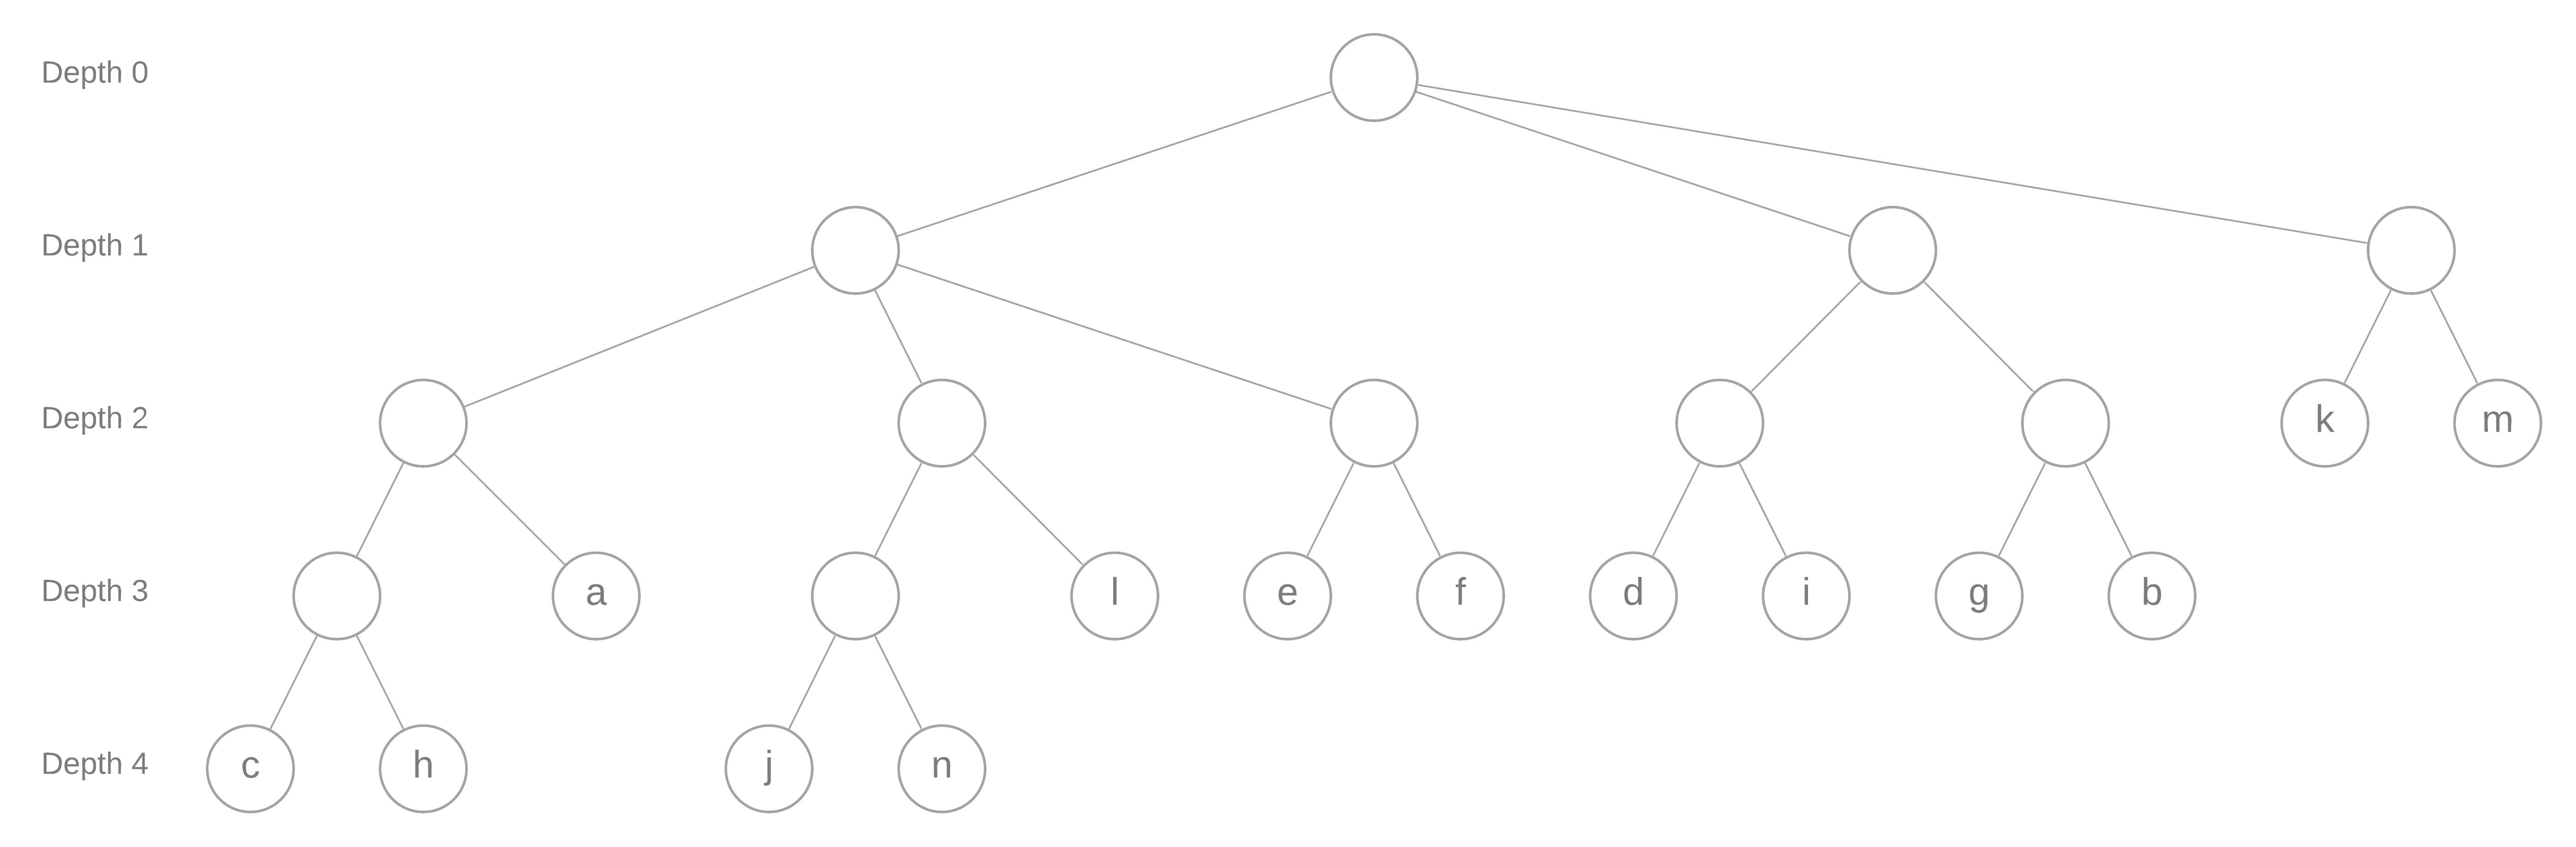
\includegraphics[width=\textwidth]{buildrun}


\begin{landscape}
\subsection{Reversing BUILD}
This algorithm has been implemented in Python 3.9, and is also included as a .py file alongside this PDF.
\begin{lstlisting}
class Constraint:
  """Class representing a tree constraint such as those used by the BUILD algorithm.
  Stored constraint becomes (a, b) < (c, d) where a, b, c, d are the four arguments provided
  """

  def __init__(self, a, b, c, d):
    self.items = [a, b, c, d]
    self.text = f'({a}, {b}) < ({c}, {d})'

class TreeNode:
  """Class representing a node in a tree. Takes two arguments:
  - children: A list of TreeNodes representing children (provide [] for a leaf)
  - name: The node's name (required for a leaf, optional otherwise)
  """

  def __init__(self, children, name=''):
    self.children = children
    self.name = name
    self.isLeaf = children == []
  
  def traverse(self):
    """Returns three values in a tuple:
    - A list of constraints representing the subtree below the current node
    - A 'flattened' list of the named nodes beneath the current node in the tree
      ie, a node with children (a node connected to (a, b), c) would return [a, b, c]
    - A list of pairs of nodes that would need to be linked together by constraints created
      by any parent of the current node
    """

    # Leaves return just themselves
    if (self.isLeaf):
      return ([], [self.name], [])
    
    numChildren = len(self.children)


    # Traverse children
    leaves = []
    internals = []

    childFlatLists = []
    constraintLists = []

    for i in self.children:
      (constraints, flatList, pairsToConnect) = i.traverse()

      if (len(flatList) == 1):
        leaves.append(flatList[0])
      
      else:
        internals.append((constraints, flatList, pairsToConnect))
        childFlatLists.append(flatList)
        constraintLists.append(constraints)

    numLeaves = len(leaves)
    numInternals = len(internals)


    # Generate constraints from data returned by children
    myConstraints = []
    myFlatList = leaves
    myPairsToConnect = []
    childPairsToConnect = []

    # If we're only connected to leaves, just return the flattened list of leaves,
    #   making sure the parent connects them
    if (numInternals == 0):
      return ([], leaves, [(leaves[i], leaves[i+1]) for i in range(numLeaves-1)])

    # If there are multiple internal children, link them all with constraints
    elif (numInternals > 1):
      # As we are connecting two internal children at a time, making one constrant for
      #   each would result in an unnecessary 'loop' - therefore we can omit one
      for i in range(numInternals-1):
        # Use the current internal child's pairsToConnect if available
        if (len(internals[i][2]) > 0):
          connectingPair = internals[i][2].pop(0)

        else:
          # Otherwise, just pick two leaves beneath it
          connectingPair = (internals[i][1][0], internals[i][1][1])
        
        # Generate constraint, adding the right hand side to the list of pairs to connect for any parent
        nextFlatList = internals[(i+1)%numInternals][1]
        myConstraints.append(Constraint(connectingPair[0], connectingPair[1], connectingPair[0], nextFlatList[0]))
        myPairsToConnect.append((connectingPair[0], nextFlatList[0]))

        # Add any remaining pairsToConnect from the current internal to a central list
        childPairsToConnect.extend(internals[i][2])
    
    # Add pairsToConnect for any children not covered above
    #   (either a single internal child skipped by the if, or the final one which was not covered by the loop)
    childPairsToConnect.extend(internals[numInternals-1][2])
    
    # Link any leaves to an internal
    # (If we've got this far without returning, we have at least one internal child)
    firstFlatList = internals[0][1]
    for i in leaves:
      # If we still have pairsToConnect from internal children, use those
      if (len(childPairsToConnect) > 0):
        connectingPair = childPairsToConnect.pop(0)
      
      else:
        # Otherwise, just use the first two leaves in the first internal
        connectingPair = firstFlatList
      
      # Generate constraint, adding the right hand side to the list of pairs to connect for any parent
      myConstraints.append(Constraint(connectingPair[0], connectingPair[1], connectingPair[0], i))
      myPairsToConnect.append((connectingPair[0], i))
    
    # If there are any more pairsToConnect from children
    while (len(childPairsToConnect) > 0):
      toConnect = childPairsToConnect.pop(0)

      # If we have any leaves, just connect to the first one
      if (numLeaves != 0):
        toConnectTo = leaves[0]
      
      else:
        # Otherwise, find a pair from any internal that doesn't include the pair we're connecting
        # There will always be at least two children in a valid tree, so
        #   if there are no leaves there will be enough internals
        toConnectTo = next(
          flatList[0]
          for flatList in childFlatLists
          if ((toConnect[0] not in flatList) and (toConnect[1] not in flatList))
        )
      
      # Generate the constraint
      #   (no need to add to myPairsToConnect as the right hand side is superfluous)
      myConstraints.append(Constraint(toConnect[0], toConnect[1], toConnect[0], toConnectTo))
    
    # Prepare output & return
    for i in childFlatLists:
      myFlatList.extend(i)
    
    for i in constraintLists:
      myConstraints.extend(i)

    return (myConstraints, myFlatList, myPairsToConnect)
  
  def getConstraints(self):
    """Returns a list of constraints representing the (sub)tree under the current node
    (Executes traverse() and returns only the constraints)
    """

    return self.traverse()[0]
\end{lstlisting}
\end{landscape}

\end{document}
